\documentclass{beamer}

\usepackage{graphicx}
\usepackage{caption}

\begin{document}
	
	\begin{frame}[plain]
		\begin{figure}
			\centering
			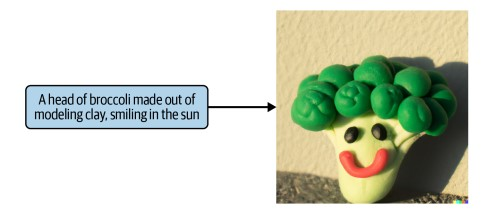
\includegraphics[width=\textwidth,height=0.85\textheight,keepaspectratio]{131.jpg}
			\caption{An example of text-to-image generation by DALL.E 2}
		\end{figure}
	\end{frame}

	\begin{frame}[plain]
		\begin{figure}
			\centering
			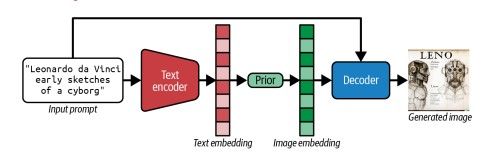
\includegraphics[width=\textwidth,height=0.85\textheight,keepaspectratio]{132.jpg}
			\caption{The DALL.E 2 architecture}
		\end{figure}
	\end{frame}
	
	
	\begin{frame}[plain]
		\begin{figure}
			\centering
			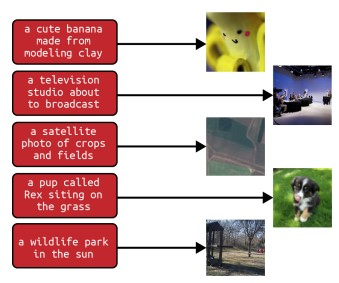
\includegraphics[width=\textwidth,height=0.85\textheight,keepaspectratio]{133.jpg}
			\caption{Examples of text–image pairs}
		\end{figure}
	\end{frame}
	
	
	\begin{frame}[plain]
		\begin{figure}
			\centering
			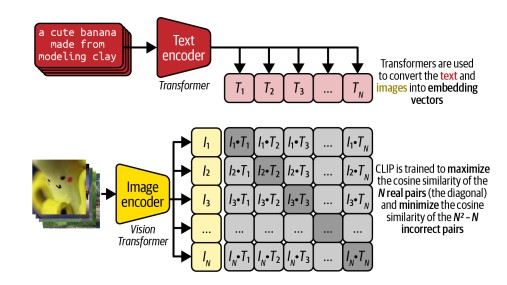
\includegraphics[width=\textwidth,height=0.85\textheight,keepaspectratio]{134.jpg}
			\caption{The CLIP training process}
		\end{figure}
	\end{frame}
	
	
	\begin{frame}[plain]
		\begin{figure}
			\centering
			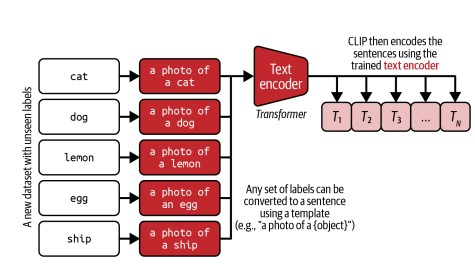
\includegraphics[width=\textwidth,height=0.85\textheight,keepaspectratio]{135.jpg}
			\caption{Converting labels in a new dataset to captions, in order to produce CLIP
				text embeddings}
		\end{figure}
	\end{frame}
	
	\begin{frame}[plain]
		\begin{figure}
			\centering
			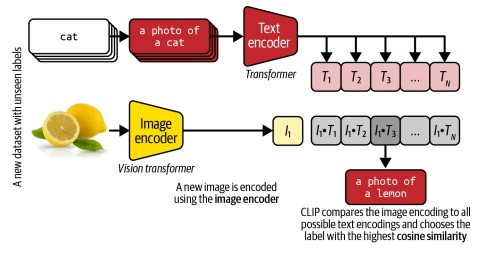
\includegraphics[width=\textwidth,height=0.85\textheight,keepaspectratio]{136.jpg}
			\caption{Using CLIP to predict the content of an image}
		\end{figure}
	\end{frame}
	
	\begin{frame}[plain]
		\begin{figure}
			\centering
			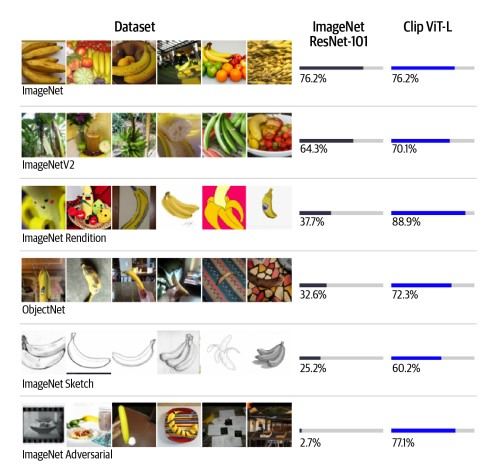
\includegraphics[width=\textwidth,height=0.85\textheight,keepaspectratio]{137.jpg}
			\caption{CLIP performs well on a wide range of image labeling datasets}
		\end{figure}
	\end{frame}
	
	
	\begin{frame}[plain]
		\begin{figure}
			\centering
			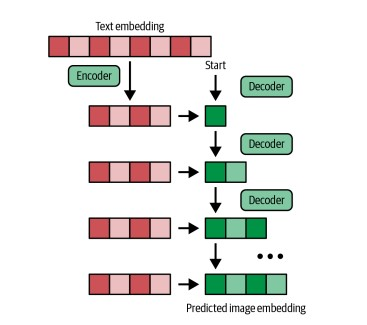
\includegraphics[width=\textwidth,height=0.85\textheight,keepaspectratio]{138.jpg}
			\caption{A simplified diagram of the autoregressive prior of DALL.E 2}
		\end{figure}
	\end{frame}
	
	
	\begin{frame}[plain]
		\begin{figure}
			\centering
			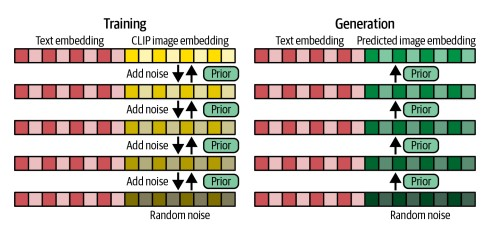
\includegraphics[width=\textwidth,height=0.85\textheight,keepaspectratio]{139.jpg}
			\caption{A simplified diagram of the diffusion prior training and generation process
				of DALL.E 2}
		\end{figure}
	\end{frame}
	
	\begin{frame}[plain]
		\begin{figure}
			\centering
			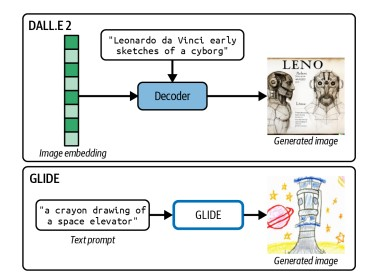
\includegraphics[width=\textwidth,height=0.78\textheight,keepaspectratio]{1310.jpg}
			\caption{A comparison between DALL.E 2 and GLIDE—GLIDE trains the entire
				generative model from scratch, whereas DALL.E 2 makes use of CLIP embeddings to
				carry information forward from the initial text prompt}
		\end{figure}
	\end{frame}
	
	\begin{frame}[plain]
		\begin{figure}
			\centering
			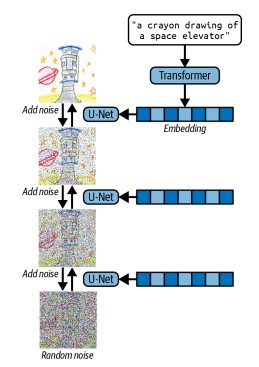
\includegraphics[width=\textwidth,height=0.85\textheight,keepaspectratio]{1311.jpg}
			\caption{The GLIDE diffusion process}
		\end{figure}
	\end{frame}
	
	
	\begin{frame}[plain]
		\begin{figure}
			\centering
			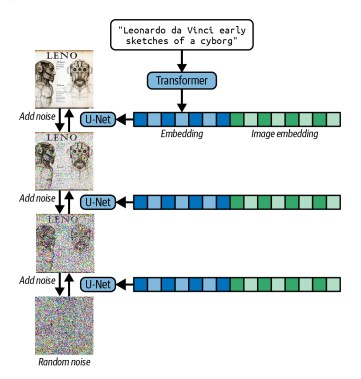
\includegraphics[width=\textwidth,height=0.85\textheight,keepaspectratio]{1312.jpg}
			\caption{The DALL.E 2 decoder additionally conditions on the image embedding
				produced by the prior}
		\end{figure}
	\end{frame}
	
	\begin{frame}[plain]
		\begin{figure}
			\centering
			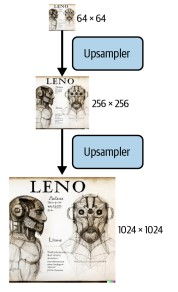
\includegraphics[width=\textwidth,height=0.74\textheight,keepaspectratio]{1313.jpg}
			\caption{The first Upsampler diffusion model converts the image from 64 × 64 pix‐
				els to 256 × 256 pixels while the second converts from 256 × 256 pixels to 1,024 × 1,024
				pixels}
		\end{figure}
	\end{frame}
	
	\begin{frame}[plain]
		\begin{figure}
			\centering
			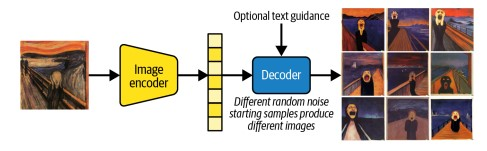
\includegraphics[width=\textwidth,height=0.85\textheight,keepaspectratio]{1314.jpg}
			\caption{DALL.E 2 can be used for generating variations of a given image}
		\end{figure}
	\end{frame}
	
	\begin{frame}[plain]
		\begin{figure}
			\centering
			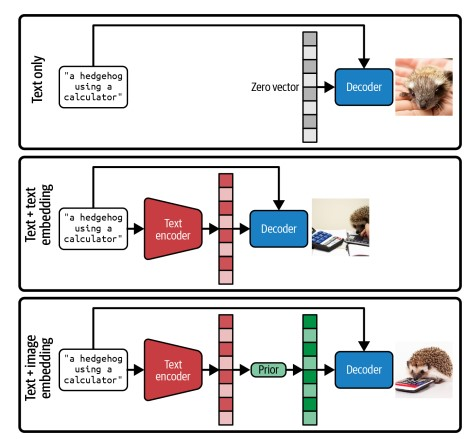
\includegraphics[width=\textwidth,height=0.85\textheight,keepaspectratio]{1315.jpg}
			\caption{The prior provides the model with additional context and helps the
				decoder to produce more accurate generations}
		\end{figure}
	\end{frame}
	
	\begin{frame}[plain]
		\begin{figure}
			\centering
			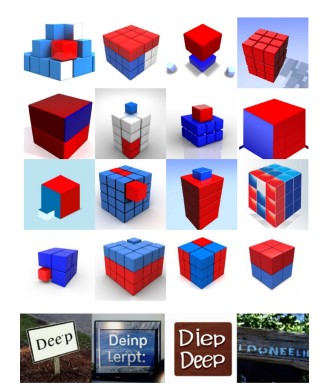
\includegraphics[width=\textwidth,height=0.78\textheight,keepaspectratio]{1316.jpg}
			\caption{Two limitations of DALL.E 2 lie in its ability to bind attributes to objects
				and reproduce textual information—top prompt: “A red cube on top of a blue cube”; bot‐
				tom prompt: “A sign that says deep learning”}
		\end{figure}
	\end{frame}
	
	\begin{frame}[plain]
		\begin{figure}
			\centering
			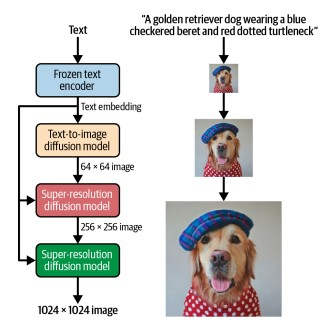
\includegraphics[width=\textwidth,height=0.85\textheight,keepaspectratio]{1317.jpg}
			\caption{The Imagen architecture}
		\end{figure}
	\end{frame}
	
	\begin{frame}[plain]
		\begin{figure}
			\centering
			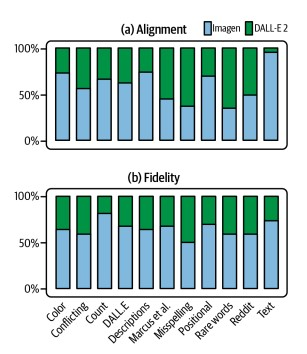
\includegraphics[width=\textwidth,height=0.85\textheight,keepaspectratio]{1318.jpg}
			\caption{Comparison of Imagen and DALL.E 2 on DrawBench across alignment
				and image fidelity}
		\end{figure}
	\end{frame}
	
	\begin{frame}[plain]
		\begin{figure}
			\centering
			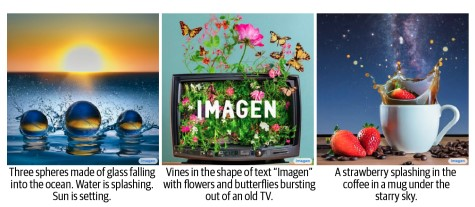
\includegraphics[width=\textwidth,height=0.85\textheight,keepaspectratio]{1319.jpg}
			\caption{Example Imagen generations}
		\end{figure}
	\end{frame}
	
	\begin{frame}[plain]
		\begin{figure}
			\centering
			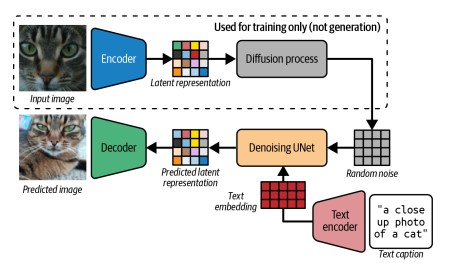
\includegraphics[width=\textwidth,height=0.85\textheight,keepaspectratio]{1320.jpg}
			\caption{The Stable Diffusion architecture}
		\end{figure}
	\end{frame}
	
	\begin{frame}[plain]
		\begin{figure}
			\centering
			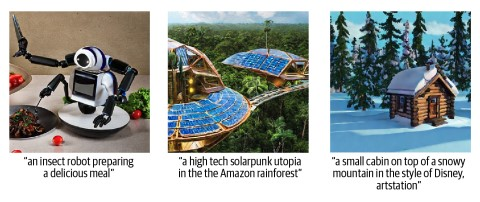
\includegraphics[width=\textwidth,height=0.85\textheight,keepaspectratio]{1321.jpg}
			\caption{Example outputs from Stable Diffusion 2.1}
		\end{figure}
	\end{frame}
	
	\begin{frame}[plain]
		\begin{figure}
			\centering
			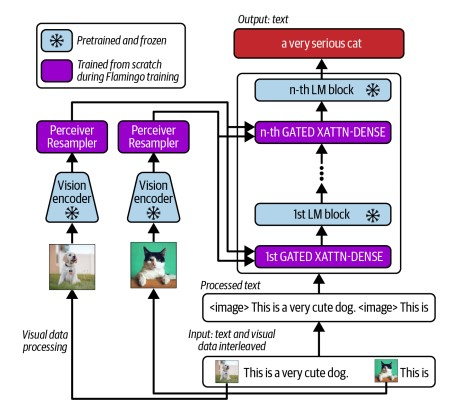
\includegraphics[width=\textwidth,height=0.85\textheight,keepaspectratio]{1322.jpg}
			\caption{The Flamingo architecture}
		\end{figure}
	\end{frame}
	
	\begin{frame}[plain]
		\begin{figure}
			\centering
			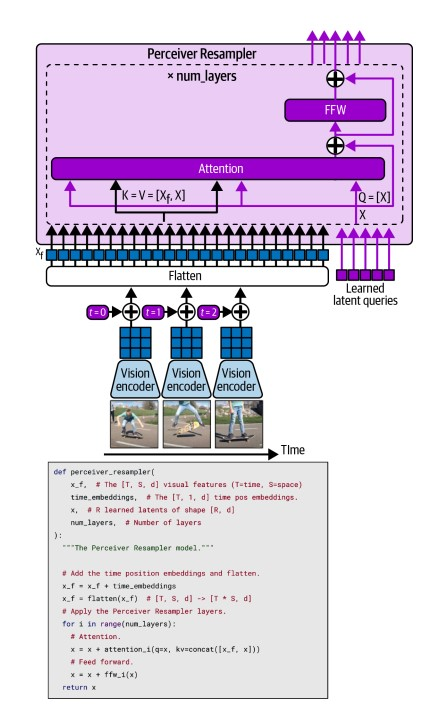
\includegraphics[width=\textwidth,height=0.85\textheight,keepaspectratio]{1323.jpg}
			\caption{The Perceiver Resampler applied to video input}
		\end{figure}
	\end{frame}
	
	\begin{frame}[plain]
		\begin{figure}
			\centering
			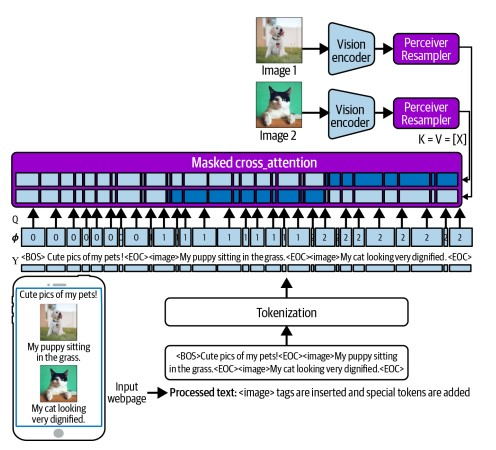
\includegraphics[width=\textwidth,height=0.85\textheight,keepaspectratio]{1324.jpg}
			\caption{Masked cross-attention (XATTN), combining vision and text data—light
				blue entries are masked and dark blue entries are nonmasked}
		\end{figure}
	\end{frame}
	
	\begin{frame}[plain]
		\begin{figure}
			\centering
			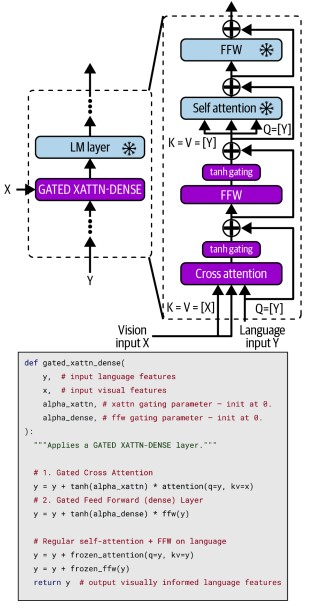
\includegraphics[width=\textwidth,height=0.85\textheight,keepaspectratio]{1325.jpg}
			\caption{A Flamingo Language Model block, comprising a frozen language model
				layer from Chinchilla and a GATED XATTN-DENSE layer}
		\end{figure}
	\end{frame}
	
	\begin{frame}[plain]
		\begin{figure}
			\centering
			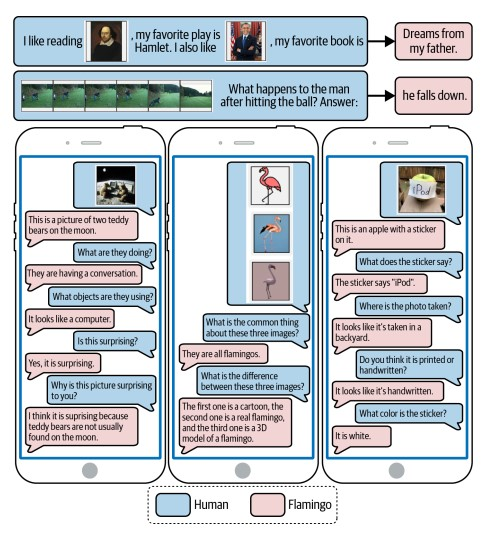
\includegraphics[width=\textwidth,height=0.85\textheight,keepaspectratio]{1326.jpg}
			\caption{Examples of inputs and outputs obtained from the 80B parameter Fla‐
				mingo model}
		\end{figure}
	\end{frame}
	
	
\end{document}